% ======================================================================
%  Mecánica Clásica usando IA — Sesión 13, Tema 3
%  Problemas de dinámica hamiltoniana
%  Codificación: UTF-8.   Compilar con pdflatex (dos veces, por el índice).
%  Duración estimada: dos sesiones de 90 min
%     Sesión 1: Problemas 1-3 ;  Sesión 2: Problemas 4-5 + actividades IA
%  Referencia: M. Cosenza, Mecánica Clásica (2024), Cap. 6.
% ======================================================================
\documentclass[spanish]{beamer}
\usepackage[utf8]{inputenc}
\usepackage[spanish]{babel}      % define \sen y usa coma decimal
\usepackage{amsmath,amssymb,mathtools}
\usepackage{graphicx}
\usepackage{textpos}
\usepackage{tikz}

\usetheme{Madrid}
\usecolortheme{beaver}
\setbeamertemplate{navigation symbols}{}

% ---------------------------------------------------------------------
%  Logo (cambie sólo esta ruta; si el archivo no existe, se omite)
% ---------------------------------------------------------------------
\newcommand{\logopath}{/Users/luisnunez/Dropbox/MisDocumentos/UIS/UISImagenInstitucional/UISLOGO.png}
\newcommand{\logoUIS}{\IfFileExists{\logopath}{\includegraphics[height=0.4in]{\logopath}}{}}
\addtobeamertemplate{frametitle}{}{%
  \begin{textblock*}{100mm}(.85\textwidth,-1cm)\logoUIS\end{textblock*}}

% ---------------------------------------------------------------------
%  Notación unificada del curso
%  L caligráfica: lagrangiano;  H caligráfica: hamiltoniano;
%  L (recta): momento angular;  sen: babel-spanish
% ---------------------------------------------------------------------
\providecommand{\sen}{\operatorname{sen}}
\newcommand{\Lag}{\mathcal{L}}
\newcommand{\Ham}{\mathcal{H}}
\newcommand{\pd}[2]{\frac{\partial #1}{\partial #2}}
\newcommand{\pb}[2]{\left\{#1,#2\right\}}   % Cosenza escribe [f,g]

% ---------------------------------------------------------------------
\title[Problemas: dinámica hamiltoniana]{\textbf{Problemas de dinámica hamiltoniana}}
\subtitle{Transformada de Legendre, transformaciones canónicas y constantes de movimiento}
\author[L.A. Núñez]{\textbf{Luis A. Núñez}}
\institute[UIS]{\textit{Escuela de Física, Facultad de Ciencias,} \\
  \textit{Universidad Industrial de Santander, Santander, Colombia} \\
  \logoUIS}
\date{\today}

\begin{document}

\begin{frame}
  \titlepage
\end{frame}

\begin{frame}{Agenda}
  \tableofcontents
\end{frame}

% ======================================================================
\section{Objetivos y convenciones}
% ======================================================================

\begin{frame}{Objetivos de la sesión}
Al finalizar, el estudiante podrá:
\begin{enumerate}
  \item<1-> \textbf{Construir} $\Ham$ a partir de $\Lag$ mediante la transformada de
        Legendre y \textbf{detectar} cuándo esa transformada es singular.
  \item<2-> \textbf{Verificar} si una transformación $(q,p)\to(Q,P)$, posiblemente
        dependiente de $t$, es canónica.
  \item<3-> \textbf{Obtener} funciones generadoras de tipo $F_1$ y $F_2$ y
        \textbf{explicar} el dominio de validez de cada una.
  \item<4-> \textbf{Relacionar} lagrangianos equivalentes
        ($\Lag \to \Lag + d\Lambda/dt$) con transformaciones canónicas.
  \item<5-> \textbf{Identificar} constantes de movimiento con paréntesis de Poisson
        y \textbf{usarlas} para reducir un problema.
\end{enumerate}
\vspace{0.2cm}
\onslide<6->{\textbf{Prerrequisitos:} ecuaciones de Euler--Lagrange, coordenadas cíclicas,
  ecuaciones de Hamilton, paréntesis de Poisson, transformaciones canónicas
  (Cosenza, Cap.~6, Secs.~6.4--6.5).}
\end{frame}

\begin{frame}{Notación y convenciones del curso}
\small
\begin{block}{Hamiltoniano y paréntesis de Poisson}
\[
  \Ham(q,p,t) = \sum_i p_i\dot q_i - \Lag , \qquad
  \frac{df}{dt} = \pb{f}{\Ham} + \pd{f}{t},
\]
\[
  \pb{f}{g} = \sum_i \left( \pd{f}{q_i}\pd{g}{p_i} - \pd{f}{p_i}\pd{g}{q_i} \right).
\]
\end{block}
\begin{block}{Funciones generadoras ($\Ham'$ es el nuevo hamiltoniano)}
\[
  F_1(q,Q,t):\ p=\pd{F_1}{q},\ P=-\pd{F_1}{Q};
  \qquad
  F_2(q,P,t):\ p=\pd{F_2}{q},\ Q=\pd{F_2}{P};
\]
\[
  \Ham' = \Ham + \partial F/\partial t \quad (F = F_1 \text{ o } F_2).
\]
\end{block}
Un grado de libertad: $(q,p)\to(Q,P)$ es canónica $\iff \pb{Q}{P}_{q,p}=1$
para todo $t$.\\
{\footnotesize $\Lag$, $\Ham$ caligráficas; $L$ (recta): momento angular.
Cosenza escribe $[f,g]$ para $\pb{f}{g}$.}
\end{frame}

\begin{frame}{Política de uso de IA en esta sesión}
\begin{itemize}
  \item<1-> \textbf{IA prohibida:} la resolución en clase de los Problemas 1--5
        y los chequeos conceptuales. Es donde se desarrolla la destreza.
  \item<2-> \textbf{IA con análisis crítico requerido:} las Actividades 1--4.
        La IA produce una respuesta; usted la audita con las herramientas de la
        física (dimensiones, límites, conservación, ecuaciones de Hamilton).
  \item<3-> \textbf{IA asistida:} los problemas \emph{Para la discusión}. Puede delegar
        álgebra verificable y depuración de código; conserva el planteamiento,
        la elección de variables y la interpretación.
  \item<4-> En todos los casos se entrega la \textbf{bitácora 4D}: prompts, respuesta,
        qué se aceptó/rechazó/corrigió, cómo se verificó y razonamiento final.
\end{itemize}
\end{frame}

% ======================================================================
\section{Problema 1: péndulo con soporte sobre una parábola}
% ======================================================================

\begin{frame}{Problema 1: el enunciado}
\small
\begin{columns}
\begin{column}{0.55\textwidth}
El punto de suspensión de un péndulo de longitud $l$ y masa $m$ se mueve sin
fricción sobre la parábola $y=ax^2$ en un plano vertical. Al soporte le
asignamos una masa $M$.
\begin{itemize}
  \item<2-> Encontrar $\Lag$ y $\Ham$.
  \item<3-> Identificar las cantidades conservadas.
  \item<4-> Analizar el límite $M\to 0$ (soporte sin masa), que es el caso del
        enunciado original (Cosenza, Prob.~6.12).
\end{itemize}
\onslide<5->{\textbf{Grados de libertad:} 2 masas en el plano (4 coordenadas)
  menos 2 ligaduras holónomas (soporte sobre $y=ax^2$; varilla rígida)
  $\Rightarrow$ 2 coordenadas generalizadas: $(x,\theta)$.}
\end{column}
\begin{column}{0.42\textwidth}
\begin{tikzpicture}[scale=1.25]
  \draw[->] (-1.6,0) -- (1.8,0) node[right] {$x$};
  \draw[->] (0,-1.0) -- (0,1.6) node[above] {$y$};
  \draw[thick,blue,domain=-1.5:1.5,smooth] plot (\x,{0.6*\x*\x});
  \node[blue] at (-1.25,1.55) {$y=ax^2$};
  \coordinate (S) at (0.8,0.384);
  \coordinate (B) at (1.4,-0.655);
  \draw[dashed] (S) -- (0.8,-0.85);
  \draw[thick] (S) -- (B) node[midway,right] {$l$};
  \draw (0.8,0.0) arc (-90:-60:0.384) node[midway,below] {\small $\theta$};
  \fill[gray] (S) circle (0.07) node[above left] {$M$};
  \fill[red] (B) circle (0.10) node[right] {$m$};
\end{tikzpicture}
{\tiny \textcolor{red}{\url{https://shorturl.at/DcEGN}}}
% Alternativa: 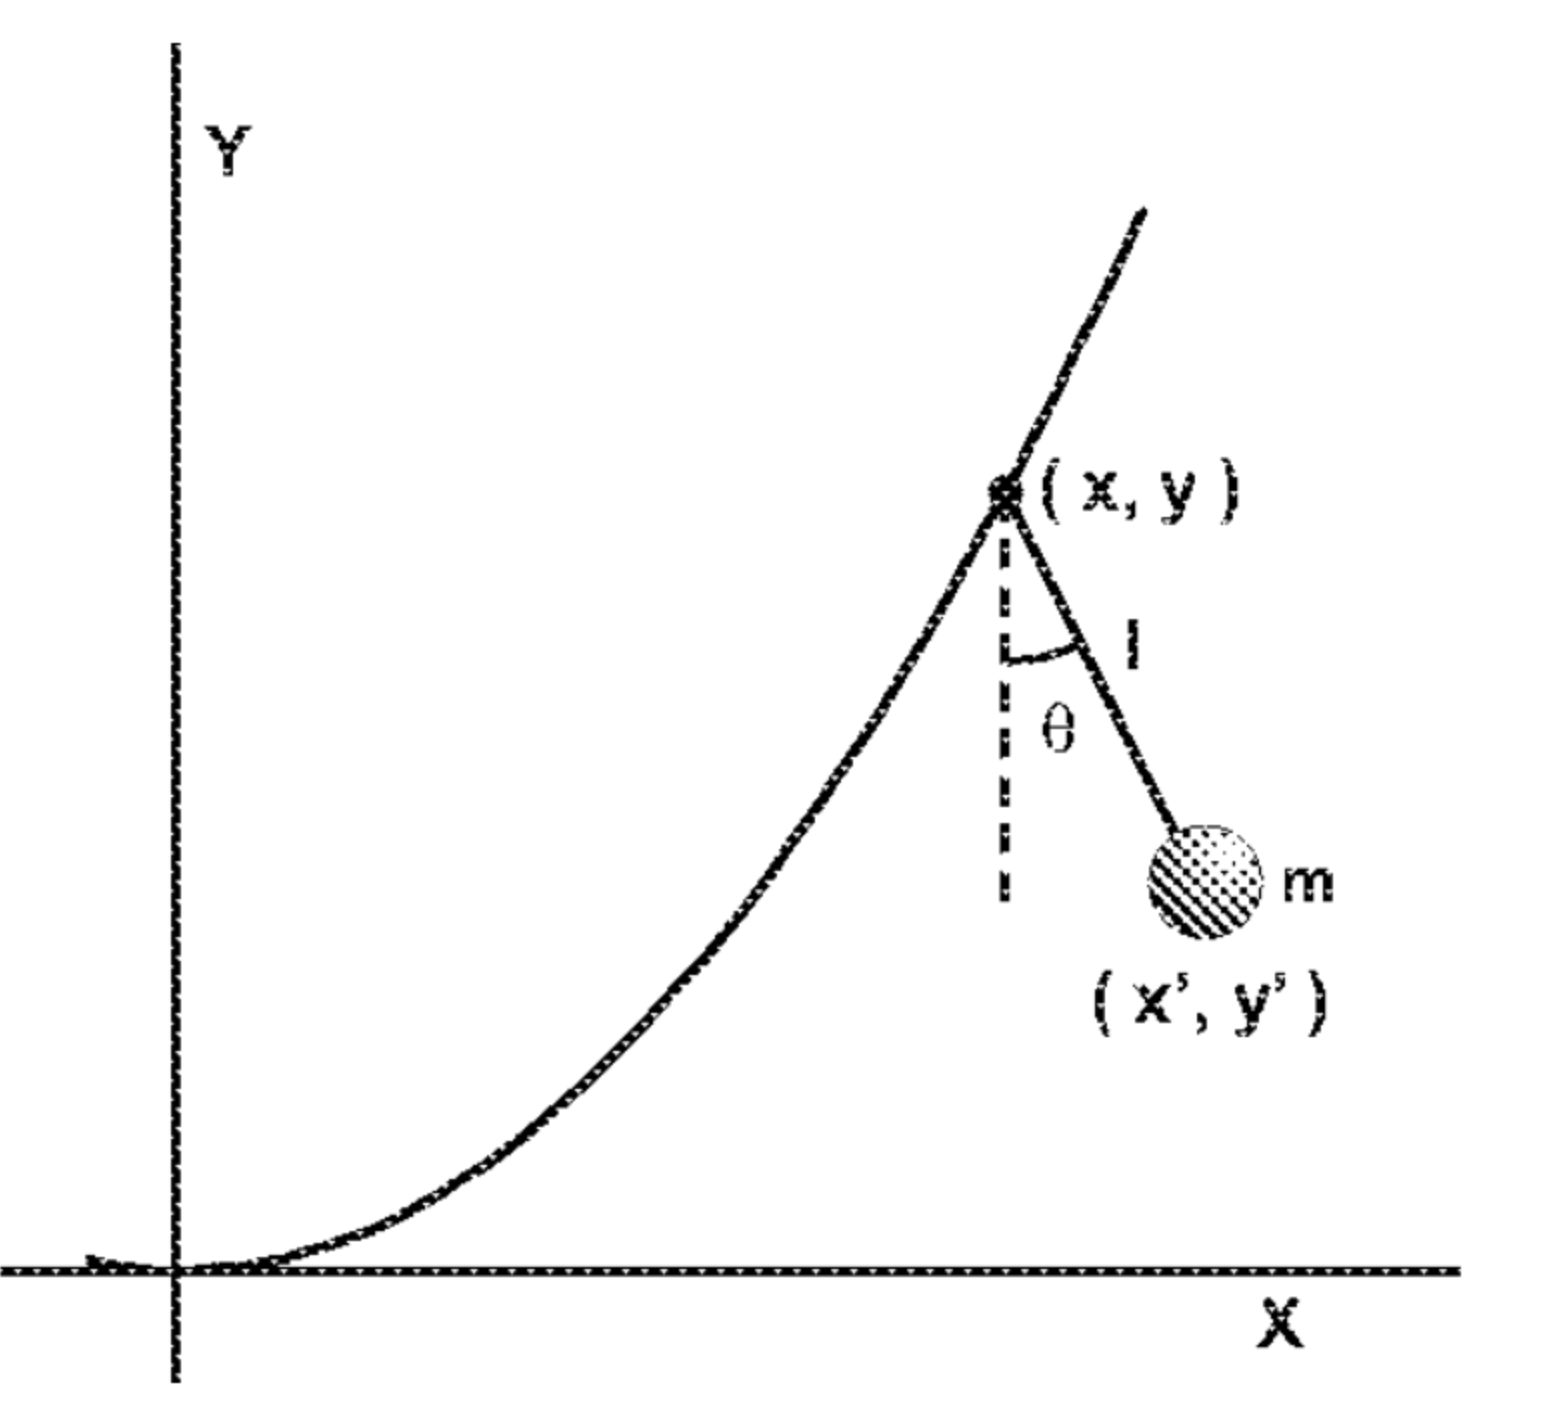
\includegraphics[width=1.8in]{Figuras/PenduloCurva.png}
\end{column} 
\end{columns}

\end{frame}

\begin{frame}{Problema 1: coordenadas, energías y lagrangiano}
Soporte en $(x,\,ax^2)$; masa $m$ en $(x',y')$:
\[
  x' = x + l\sen\theta, \qquad y' = ax^2 - l\cos\theta ,
\]
\[
  \dot x' = \dot x + l\dot\theta\cos\theta, \qquad
  \dot y' = 2ax\dot x + l\dot\theta\sen\theta .
\]
\pause
Conviene definir tres funciones de la configuración:
\[
  \sigma = 1+4a^2x^2, \quad
  \kappa = \cos\theta + 2ax\sen\theta, \quad
  D = \sen\theta - 2ax\cos\theta .
\]
\pause
\[
  T = \tfrac12 (M+m)\,\sigma\,\dot x^2 + m l\,\kappa\,\dot x\dot\theta
      + \tfrac12 m l^2 \dot\theta^2 ,
\]
\[
  V = (M+m)\,g\,a x^2 - m g l \cos\theta , \qquad \Lag = T - V .
\]
\pause
\textbf{Chequeos:} cada término de $T$ tiene dimensiones de energía
($[a]=\text{longitud}^{-1}$); con $a=0$ se recupera el péndulo con soporte
deslizante sobre una recta horizontal.
\end{frame}

\begin{frame}{Problema 1: la transformada de Legendre}
$T$ es una forma cuadrática en las velocidades,
$T=\tfrac12\,\dot{\mathbf q}^{\mathsf T}\mathsf M\,\dot{\mathbf q}$, con
$\dot{\mathbf q}=(\dot x,\dot\theta)^{\mathsf T}$ y
\[
  \mathsf M = \begin{pmatrix} (M+m)\sigma & m l \kappa \\ m l\kappa & m l^2 \end{pmatrix},
  \qquad
  \begin{pmatrix} p_x \\ p_\theta \end{pmatrix} = \mathsf M
  \begin{pmatrix} \dot x \\ \dot\theta \end{pmatrix}.
\]
\pause
Usando la identidad $\kappa^2 + D^2 = \sigma$ (verifíquela):
\[
  \det \mathsf M = m l^2 \left[ (M+m)\sigma - m\kappa^2 \right]
                 = m l^2 \left[ M\sigma + m D^2 \right] .
\]
\pause
\begin{itemize}
  \item Si $M>0$: $\det\mathsf M>0$ en toda la configuración; las velocidades se
        despejan siempre: $\dot{\mathbf q}=\mathsf M^{-1}\mathbf p$.
  \item Si $M=0$: $\det\mathsf M = m^2l^2D^2$ \alert{se anula cuando $D=0$}.
\end{itemize}
\end{frame}

\begin{frame}{Problema 1: el hamiltoniano}
Como la ligadura no depende de $t$ y $T$ es cuadrática homogénea en las
velocidades, $\Ham = \tfrac12\,\mathbf p^{\mathsf T}\mathsf M^{-1}\mathbf p + V = T+V$:
\[
  \Ham = \frac{m l^2 p_x^2 - 2 m l\,\kappa\, p_x p_\theta + (M+m)\,\sigma\, p_\theta^2}
              {2 m l^2 \left( M\sigma + m D^2 \right)}
         + (M+m)\,g\,a x^2 - m g l\cos\theta .
\]
\pause
\begin{itemize}
  \item<2-> $\partial\Ham/\partial t = 0 \Rightarrow \Ham = E$ se conserva.
  \item<3-> $\Ham$ depende de $x$ y de $\theta$: \textbf{no hay coordenadas cíclicas}.
        Con $a=0$, $x$ se vuelve cíclica y $p_x$ (momento horizontal total) se conserva.
  \item<4-> Las ecuaciones de Hamilton $\dot x = \partial\Ham/\partial p_x$, \ldots,
        $\dot p_\theta = -\partial\Ham/\partial\theta$ son largas: es una tarea
        \textbf{delegable y verificable} (Actividad 1).
\end{itemize}
\end{frame}

\begin{frame}{Problema 1: el límite de soporte sin masa ($M\to 0$)}
\[
  \Ham_{M=0} = \frac{p_x^2}{2mD^2} - \frac{\kappa\,p_x p_\theta}{m l D^2}
             + \frac{\sigma\,p_\theta^2}{2 m l^2 D^2} + m g\left(a x^2 - l\cos\theta\right)
\]
\pause
\begin{itemize}
  \item<2-> $D=0 \iff \tan\theta = 2ax$: la varilla es \textbf{normal} a la parábola.
        Ahí el soporte puede moverse a lo largo de la tangente mientras la varilla
        rota, de modo que la masa $m$ queda instantáneamente en reposo:
        hay velocidades $(\dot x,\dot\theta)\neq 0$ con $T=0$.
  \item<3-> ¡El equilibrio $x=0,\ \theta=0$ satisface $D=0$! El hamiltoniano del
        soporte sin masa es singular justamente donde queremos estudiar
        pequeñas oscilaciones.
  \item<4-> Lección: la transformada de Legendre exige
        $\det\left(\partial^2\Lag/\partial\dot q_i\partial\dot q_j\right)\neq 0$.
        Un modelo con un grado de libertad sin inercia lo viola.
        La masa $M$ regulariza el problema.
\end{itemize}
\end{frame}
% NOTA DOCENTE: la versión anterior de estas diapositivas daba
%   H = px^2/(2m D^2) + p_theta^2 sigma/(2 m l^2 D^2),
% sin el término cruzado -kappa px ptheta/(m l D^2) y sin V. Se usa en la
% Actividad 1 como respuesta a auditar.

% ======================================================================
\section{Problema 2: \texorpdfstring{$\Ham = q + t e^p$}{H = q + t exp(p)}}
% ======================================================================

\begin{frame}{Problema 2: el enunciado y la condición canónica}
El hamiltoniano de un sistema (variables adimensionales) es $\Ham = q + t\,e^{p}$.
Mostrar que $Q = q + e^{p}$, $P = p$ es canónica; hallar su función generadora;
obtener $\Ham'$ y resolver las ecuaciones de movimiento.
\pause
\begin{itemize}
  \item<2-> Con un grado de libertad, $\pb{Q}{Q}=\pb{P}{P}=0$ se cumplen siempre
        por antisimetría. La única condición es
  \[
    \pb{Q}{P}_{q,p} = \pd{Q}{q}\pd{P}{p} - \pd{Q}{p}\pd{P}{q}
                    = (1)(1) - (e^{p})(0) = 1 . \qquad \checkmark
  \]
  \item<3-> Equivalentemente, el jacobiano $\partial(Q,P)/\partial(q,p)=1$:
        la transformación conserva el área en el espacio de fase.
\end{itemize}
\end{frame}

\begin{frame}{Problema 2: la función generadora $F_2(q,P)$}
Buscamos $F_2(q,P)$ con $p = \partial F_2/\partial q$ y $Q = \partial F_2/\partial P$.
\begin{itemize}
  \item<2-> Escribimos $Q$ en las variables de $F_2$: $Q = q + e^{P}$. Integrando en $P$,
  \[
    F_2(q,P) = qP + e^{P} + g(q) ,
  \]
  donde la ``constante'' de integración es una \alert{función arbitraria de $q$}.
  \item<3-> La fija la otra relación:
  $p = \partial F_2/\partial q = P + g'(q)$, y como $p=P$, $g'(q)=0$.
  \item<4-> Resultado (salvo una constante aditiva irrelevante):
  \[
    F_2(q,P) = qP + e^{P} .
  \]
  El término $qP$ genera la identidad; $e^{P}$ produce el corrimiento
  $Q - q = e^{P}$.
\end{itemize}
\end{frame}

\begin{frame}{Problema 2: el nuevo hamiltoniano y la solución}
Como $\partial F_2/\partial t = 0$, $\Ham'(Q,P,t) = \Ham\big(q(Q,P),p(Q,P),t\big)$ con
$q = Q - e^{P}$:
\[
  \Ham' = Q + (t-1)\,e^{P} .
\]
\pause
Ecuaciones de Hamilton en las nuevas variables:
\[
  \dot P = -\pd{\Ham'}{Q} = -1 , \qquad
  \dot Q = \pd{\Ham'}{P} = (t-1)\,e^{P} .
\]
\pause
Con $P(0)=P_0$, $Q(0)=Q_0$:
\[
  P = P_0 - t, \qquad
  Q = Q_0 + e^{P_0}\!\int_0^t (s-1)e^{-s}ds = Q_0 - t\,e^{P_0 - t}.
\]
\pause
Regresando a $(q,p)$ con $q_0 = Q_0 - e^{p_0}$:
\[
  p = p_0 - t, \qquad q = q_0 + e^{p_0}\left[1 - (1+t)\,e^{-t}\right].
\]
\end{frame}

\begin{frame}{Problema 2: verificación y discernimiento}
\begin{itemize}
  \item<1-> \textbf{Verificación directa:} $\dot q = \partial\Ham/\partial p = t\,e^{p}$,
        $\dot p = -1$. Sustituya $p(t)$ y $q(t)$: ambas se cumplen y $q(0)=q_0$.
  \item<2-> \textbf{$\Ham$ no se conserva:}
        $d\Ham/dt = \pb{\Ham}{\Ham} + \partial\Ham/\partial t = e^{p}$.
        Compruébelo derivando $q+te^{p}$ a lo largo de la solución.
  \item<3-> \textbf{Dimensiones:} $q + t\,e^{p}$ sólo tiene sentido con variables
        adimensionales (o con constantes implícitas). Una respuesta de IA que no
        lo advierta debe señalarse.
  \item<4-> \textbf{¿Ganamos algo?} Aquí no: el problema era más sencillo en $(q,p)$.
        Una transformación canónica es útil cuando vuelve cíclica alguna
        coordenada. ¿Qué transformación lo lograría para este $\Ham$?
\end{itemize}
\end{frame}
% NOTA DOCENTE: una opción para la última pregunta: tomar como nuevo momento
% una constante de movimiento, p.ej. P = p + t (pues dp/dt = -1).

% ======================================================================
\section{Problema 3: hamiltonianos y lagrangianos equivalentes}
% ======================================================================

\begin{frame}{Problema 3: el enunciado y el lagrangiano}
Un sistema unidimensional tiene
\[
  \Ham = \frac{p^2}{2m} - A\left( \frac{p}{m}\cos\gamma t - \gamma q \sen\gamma t \right)
         + \frac12 k q^2 .
\]
Encontrar $\Lag$, un lagrangiano equivalente $\Lag'$ y la relación entre $\Ham$ y $\Ham'$.
\pause
\begin{itemize}
  \item<2-> De $\dot q = \partial\Ham/\partial p = p/m - (A/m)\cos\gamma t$:
  \quad $p = m\dot q + A\cos\gamma t$.
  \item<3-> Entonces $\Lag = p\dot q - \Ham$:
  \[
    \Lag = \frac12 m\dot q^2 - \frac12 k q^2 + A\dot q\cos\gamma t
           - A\gamma q\sen\gamma t + \frac{A^2}{2m}\cos^2\gamma t .
  \]
\end{itemize}
\onslide<4->{\alert{Nota:} el signo de $\gamma q\sen\gamma t$ en $\Ham$ es esencial
  (Actividad 2).}
\end{frame}

\begin{frame}{Problema 3: el lagrangiano equivalente}
\begin{itemize}
  \item<1-> Los dos términos con $A$ que dependen de $q$ forman una derivada total:
  \[
    A\dot q\cos\gamma t - A\gamma q\sen\gamma t = \frac{d}{dt}\left( A q\cos\gamma t \right),
  \]
  y el término $\frac{A^2}{2m}\cos^2\gamma t$ sólo depende de $t$.
  \item<2-> Por lo tanto $\Lag = \Lag' + d\Lambda/dt$ con
  \[
    \Lag' = \frac12 m\dot q^2 - \frac12 k q^2,
  \]
  \[
    \Lambda(q,t) = A q\cos\gamma t + \frac{A^2}{4\gamma m}
                   \left( \gamma t + \sen\gamma t\cos\gamma t \right).
  \]
  \item<3-> $\Lag$ y $\Lag'$ dan la \textbf{misma} ecuación de movimiento:
        $m\ddot q + kq = 0$. El sistema es un oscilador libre de frecuencia
        $\omega_0 = \sqrt{k/m}$.
  \item<4-> Para $\Lag'$: \ $p' = m\dot q$, \quad
        $\Ham' = \dfrac{p'^2}{2m} + \dfrac12 k q^2$.
\end{itemize}
\end{frame}

\begin{frame}{Problema 3: la relación general entre $\Ham$ y $\Ham'$}
Para cualquier $\Lag = \Lag' + d\Lambda(q,t)/dt$, con
$d\Lambda/dt = (\partial\Lambda/\partial q)\,\dot q + \partial\Lambda/\partial t$:
\begin{itemize}
  \item<2-> Momentos:
  \(
    p = \pd{\Lag}{\dot q} = \pd{\Lag'}{\dot q} + \pd{\Lambda}{q} = p' + \pd{\Lambda}{q}.
  \)
  \item<3-> Hamiltonianos:
  \[
    \Ham = p\dot q - \Lag
         = \left(p' + \pd{\Lambda}{q}\right)\dot q - \Lag'
           - \pd{\Lambda}{q}\dot q - \pd{\Lambda}{t}
         = \Ham' - \pd{\Lambda}{t} .
  \]
  \item<4-> Comprobación en nuestro caso: con $p' = p - A\cos\gamma t$ y
  $\partial\Lambda/\partial t = -A\gamma q\sen\gamma t + \frac{A^2}{2m}\cos^2\gamma t$,
  la expresión $\Ham' - \partial\Lambda/\partial t$ reproduce el $\Ham$ del enunciado.
\end{itemize}
\end{frame}

\begin{frame}{Problema 3: interpretación}
\begin{itemize}
  \item<1-> El cambio $(q,p)\to(q,p')$ es una \textbf{transformación canónica} con
  \[
    F_2(q,P,t) = qP + \Lambda(q,t)
    \;\Rightarrow\;
    p = P + \pd{\Lambda}{q},\quad Q = q,\quad
    \Ham' = \Ham + \pd{\Lambda}{t} .
  \]
  Coincide con el resultado anterior: sumar $d\Lambda/dt$ a $\Lag$ es una
  transformación canónica que no mueve la coordenada.
  \item<2-> \textbf{Momento canónico vs.\ mecánico:} $p = m\dot q + A\cos\gamma t$ es
        canónico; $p' = m\dot q$ es mecánico. Es el análogo clásico de una
        transformación de norma (\emph{gauge}).
  \item<3-> \textbf{Conservación:} $\Ham$ depende explícitamente de $t$ y no se
        conserva; $\Ham' = \frac12 m\dot q^2 + \frac12 kq^2$ sí. ``El''
        hamiltoniano de un sistema no es único: depende de las variables.
  \item<4-> Conexión: en la cuenta sobre una varilla rotante (sesión anterior)
        $\Ham$ se conserva pero no es la energía. Aquí la energía se conserva
        pero $\Ham$ no.
\end{itemize}
\end{frame}

% ======================================================================
\section{Problema 4: constantes de movimiento \texorpdfstring{$f(q_1,p_1)$}{f(q1,p1)}}
% ======================================================================

\begin{frame}{Problema 4: una función que sólo entra a través de $f$}
Sea $\Ham = \Ham\big(f(q_1,p_1),\,q_2,\ldots,q_n,\,p_2,\ldots,p_n\big)$.
Mostrar que $f$ es constante de movimiento.
\begin{itemize}
  \item<2-> $f$ no depende de $t$ ni de $(q_i,p_i)$ con $i\ge 2$, así que en
        $\pb{f}{\Ham}$ sólo sobrevive $i=1$. Por la regla de la cadena,
        $\partial\Ham/\partial q_1 = (\partial\Ham/\partial f)(\partial f/\partial q_1)$
        y lo mismo para $p_1$:
  \[
    \frac{df}{dt} = \pb{f}{\Ham}
    = \pd{\Ham}{f}\left( \pd{f}{q_1}\pd{f}{p_1} - \pd{f}{p_1}\pd{f}{q_1} \right) = 0 .
  \]
  \item<3-> Generaliza la coordenada cíclica: si $f = p_1$, entonces $q_1$ es cíclica.
  \item<4-> El resultado se aplica en cascada: si $\Ham = \Ham\big(g(q_2,p_2,f),\ldots\big)$,
        también $g$ se conserva.
\end{itemize}
\end{frame}

\begin{frame}{Problema 4: partícula en el potencial $V = \mathbf a\cdot\mathbf r/r^3$}
Con $\mathbf a = a_z\hat{\mathbf z}$ constante (potencial de un dipolo;
$[a_z] = \text{energía}\times\text{longitud}^2$), en coordenadas esféricas
$V = a_z\cos\theta/r^2$ y
\[
  \Ham = \frac{p_r^2}{2m} + \frac{p_\theta^2}{2mr^2}
       + \frac{p_\phi^2}{2mr^2\sen^2\theta} + \frac{a_z\cos\theta}{r^2} .
\]
\begin{itemize}
  \item<2-> $\phi$ es cíclica $\Rightarrow p_\phi = L_z$ se conserva (primer nivel de la cascada).
  \item<3-> Agrupando:
  \[
    \Ham = \frac{p_r^2}{2m} + \frac{f(\theta,p_\theta;p_\phi)}{2mr^2},
    \qquad
    f = p_\theta^2 + \frac{p_\phi^2}{\sen^2\theta} + 2ma_z\cos\theta .
  \]
  \item<4-> Por el resultado anterior, $f$ es constante de movimiento.
\end{itemize}
\end{frame}

\begin{frame}{Problema 4: interpretación y conexiones}
\begin{itemize}
  \item<1-> \alert{Cuidado:} la cantidad conservada es $f$, \textbf{no} $f/(2mr^2)$.
        Como $r$ varía,
        \[
          \frac{d}{dt}\left(\frac{f}{2mr^2}\right) = -\frac{p_r\, f}{m^2 r^3}\neq 0 .
        \]
  \item<2-> \textbf{Límite $a_z\to 0$:}
        $f \to p_\theta^2 + p_\phi^2/\sen^2\theta = L^2$, el cuadrado del momento
        angular. $f$ es la generalización de $L^2$ cuando la simetría esférica se
        rompe pero sobrevive la estructura $1/r^2$.
  \item<3-> \textbf{Reducción:} el movimiento radial es el de un problema
        unidimensional con $V_{\text{ef}}(r) = f/(2mr^2)$.
        ¿Qué ocurre si $f<0$?
  \item<4-> \textbf{Integrabilidad:} $\Ham$, $p_\phi$ y $f$ son tres constantes
        independientes con $\pb{\Ham}{p_\phi}=\pb{\Ham}{f}=\pb{p_\phi}{f}=0$
        (en involución): el sistema es integrable y separable en la ecuación de
        Hamilton--Jacobi (próximo tema).
\end{itemize}
\end{frame}

% ======================================================================
\section{Problema 5: una rotación en el espacio de fase}
% ======================================================================

\begin{frame}{Problema 5: el enunciado y la condición canónica}
Sea $\omega>0$ una constante y $\gamma$ otra constante con dimensiones de frecuencia.
Mostrar que
\[
  q = Q\cos\gamma t + \frac{P}{m\omega}\sen\gamma t, \qquad
  p = -m\omega Q\sen\gamma t + P\cos\gamma t
\]
es canónica; hallar $F_2(q,P,t)$; aplicarla al oscilador
$\Ham = \frac{p^2}{2m} + \frac12 m\omega^2 q^2$.
\pause
\begin{itemize}
  \item<2-> Para cada $t$ fijo:
  \[
    \pb{q}{p}_{Q,P} = \pd{q}{Q}\pd{p}{P} - \pd{q}{P}\pd{p}{Q}
    = \cos^2\gamma t + \sen^2\gamma t = 1 . \;\checkmark
  \]
  \item<3-> Geometría: en las variables $(q,\,p/m\omega)$, que tienen ambas
        dimensiones de longitud, la transformación es una \textbf{rotación rígida}
        de ángulo $\gamma t$. Conserva áreas.
\end{itemize}
\end{frame}

\begin{frame}{Problema 5: la función generadora $F_2(q,P,t)$}
\begin{itemize}
  \item<1-> Expresamos $Q$ y $p$ en las variables $(q,P)$ de $F_2$ (si $\cos\gamma t\neq 0$):
  \[
    Q = \frac{q}{\cos\gamma t} - \frac{P}{m\omega}\tan\gamma t, \qquad
    p = \frac{P}{\cos\gamma t} - m\omega q\tan\gamma t .
  \]
  \item<2-> Integramos $\partial F_2/\partial q = p$ y fijamos la función de $(P,t)$
        con $\partial F_2/\partial P = Q$:
  \[
    F_2(q,P,t) = \frac{qP}{\cos\gamma t}
                 - \frac{\tan\gamma t}{2}\left( m\omega q^2 + \frac{P^2}{m\omega} \right).
  \]
  \item<3-> Chequeo: en $t=0$, $F_2 = qP$ (la identidad), como debe ser.
\end{itemize}
\end{frame}

\begin{frame}{Problema 5: $F_1$, $F_2$ y sus dominios}
\begin{itemize}
  \item<1-> $F_2$ es singular cuando $\cos\gamma t = 0$: en $\gamma t=\pi/2$,
        $q = P/m\omega$, de modo que $q$ y $P$ \textbf{no son independientes}
        y no pueden ser las variables de $F_2$.
  \item<2-> Allí sirve $F_1(q,Q,t) = F_2 - QP$ (con $P$ expresado en $q,Q$):
  \[
    F_1(q,Q,t) = \frac{m\omega}{2\sen\gamma t}
                 \left[ \left(q^2 + Q^2\right)\cos\gamma t - 2qQ \right],
  \]
  con $p = \partial F_1/\partial q$ y $P = -\partial F_1/\partial Q$ (verifíquelo).
  \item<3-> $F_1$ falla en $\sen\gamma t = 0$; en particular en $t=0$, porque la
        identidad ($Q=q$) no admite una función de tipo $F_1$.
  \item<4-> Lección: el \emph{tipo} de función generadora es una elección de
        variables independientes; la transformación canónica es la misma.
\end{itemize}
\end{frame}

\begin{frame}{Problema 5: el nuevo hamiltoniano}
\begin{itemize}
  \item<1-> Sustituyendo $q(Q,P,t)$ y $p(Q,P,t)$, el hamiltoniano del oscilador
        no cambia de forma (una rotación preserva el círculo):
  \[
    \Ham = \frac{P^2}{2m} + \frac12 m\omega^2 Q^2 .
  \]
  \item<2-> La derivada temporal de $F_2$, expresada en $(Q,P)$:
  \[
    \pd{F_2}{t} = -\frac{\gamma}{2}\left( m\omega Q^2 + \frac{P^2}{m\omega} \right)
                = -\frac{\gamma}{\omega}\left( \frac{P^2}{2m} + \frac12 m\omega^2 Q^2 \right).
  \]
  \item<3-> Por lo tanto
  \[
    \Ham' = \Ham + \pd{F_2}{t}
          = \left( 1 - \frac{\gamma}{\omega} \right)
            \left( \frac{P^2}{2m} + \frac12 m\omega^2 Q^2 \right).
  \]
\end{itemize}
\end{frame}

\begin{frame}{Problema 5: solución e interpretación}
\begin{itemize}
  \item<1-> Ecuaciones de Hamilton:
        $\dot Q = (1-\gamma/\omega)P/m$, \
        $\dot P = -(1-\gamma/\omega)m\omega^2 Q$
        $\Rightarrow \ddot Q = -\Omega^2 Q$, con $\Omega = \omega - \gamma$.
  \item<2-> Las nuevas variables oscilan a $\omega-\gamma$: describimos el movimiento
        desde un sistema que \textbf{rota en el espacio de fase} con frecuencia $\gamma$.
  \item<3-> \textbf{Caso $\gamma = \omega$:} $\Ham' = 0$, así que $Q = q_0$ y $P = p_0$
        son constantes y
        \[
          q(t) = q_0\cos\omega t + \frac{p_0}{m\omega}\sen\omega t .
        \]
        La transformación \emph{es} el flujo del oscilador.
  \item<4-> Con $\gamma=\omega$, $F_2$ cumple
        $\Ham\left(q,\partial F_2/\partial q\right) + \partial F_2/\partial t = 0$:
        es una solución de la \textbf{ecuación de Hamilton--Jacobi}
        (próximo tema).
\end{itemize}
\end{frame}

% ======================================================================
\section{Recapitulando}
% ======================================================================

\begin{frame}{Chequeos conceptuales (sin IA, 10 minutos)}
\begin{enumerate}
  \item<1-> En el Problema 1, $\Ham = E$; en el 3, $\Ham \neq$ cte; en la cuenta
        sobre la varilla rotante, $\Ham=$ cte $\neq E$. ¿Qué dos condiciones
        separan estos casos?
  \item<2-> Si $\pb{Q}{P}=1$ para todo $t$ pero la transformación depende de $t$,
        ¿por qué $\Ham'\neq\Ham(q(Q,P),p(Q,P))$?
  \item<3-> ¿Puede una transformación ser canónica y no admitir una $F_2$?
        Dé un ejemplo de esta sesión.
  \item<4-> Un compañero afirma: ``en el Problema 4, $p_\theta$ se conserva porque
        $\theta$ aparece sólo dentro de $f$''. ¿Es correcto?
  \item<5-> En el Problema 1 con $M=0$, $\det\mathsf M=0$ si $D=0$. ¿Afecta esto sólo
        a la formulación hamiltoniana o también a las ecuaciones de
        Euler--Lagrange? Justifique.
\end{enumerate}
\end{frame}
% NOTA DOCENTE (respuestas breves):
% 1. Ligaduras independientes de t y T cuadrática homogénea => H=E;
%    dH/dt = dH/dt parcial => H=cte si no depende explícitamente de t.
% 2. Porque H' = H + dF/dt: la transformación misma "se mueve".
% 3. Sí: Problema 5 en gamma t = pi/2 (q y P no independientes).
% 4. No: se conserva f, no p_theta; dp_theta/dt = -(dH/df) df/dtheta != 0.
% 5. A ambas: E-L se escriben M qddot = (fuerzas); si det M = 0 las
%    aceleraciones no quedan determinadas. Es una propiedad del modelo,
%    no de la formulación (ver Para la discusión 3/3).

\begin{frame}{Recapitulando}
\begin{itemize}
  \item<1-> $\Ham = \tfrac12\mathbf p^{\mathsf T}\mathsf M^{-1}\mathbf p + V$ exige
        $\det\mathsf M\neq 0$. Grados de libertad sin inercia hacen singular la
        transformada de Legendre.
  \item<2-> Canonicidad (un grado de libertad): $\pb{Q}{P}=1$. Función generadora:
        integrar una relación y fijar la ``constante'' con la otra.
  \item<3-> $\Lag\to\Lag + d\Lambda/dt$ \ $\Leftrightarrow$ \
        $F_2 = qP + \Lambda$, \ $\Ham' = \Ham + \partial\Lambda/\partial t$.
        $\Ham$ depende de la elección de variables.
  \item<4-> Si $\Ham$ depende de $(q_1,p_1)$ sólo a través de $f$, entonces $f$ se
        conserva; aplicado en cascada lleva a la integrabilidad.
  \item<5-> Una transformación canónica dependiente de $t$ con $\Ham'=0$ es el
        propio flujo; su $F_2$ resuelve la ecuación de Hamilton--Jacobi.
\end{itemize}
\vspace{0.2cm}
\onslide<6->{\textbf{Próximo tema:} ecuación de Hamilton--Jacobi, separación de
  variables y variables de acción--ángulo.}
\end{frame}

% ======================================================================
\section{Actividades con IA (modelo 4D)}
% ======================================================================

\begin{frame}{Actividad 1 (Discernimiento): auditar un hamiltoniano}
Para el Problema 1 con $M=0$, un asistente de IA propone
\[
  \Ham_{\text{IA}} = \frac{p_x^2}{2mD^2} + \frac{\sigma\,p_\theta^2}{2ml^2D^2} .
\]
\begin{itemize}
  \item<2-> \textbf{Delegación:} usted conserva $T$, $V$ y la matriz $\mathsf M$;
        puede delegar la inversión de $\mathsf M$.
  \item<3-> \textbf{Discernimiento:} sin rehacer todo, encuentre al menos dos
        pruebas que lo refuten:
        (i) $\dot x = \partial\Ham/\partial p_x$ frente a $\mathsf M^{-1}\mathbf p$;
        (ii) ¿qué da $\Ham_{\text{IA}}$ para $\mathbf p = 0$?;
        (iii) ¿es $\Ham_{\text{IA}} = T+V$?
  \item<4-> \textbf{Descripción:} redacte un prompt que obligue al asistente a
        incluir la gravedad, los términos cruzados y a reportar $\det\mathsf M$.
  \item<5-> \textbf{Diligencia:} pida las ecuaciones de Hamilton para $M>0$ y
        verifique con SymPy que $d\Ham/dt = 0$ a lo largo de ellas.
\end{itemize}
\end{frame}

\begin{frame}{Actividad 2 (Descripción): un signo cambia la física}
Pida a un asistente de IA que resuelva el Problema 3 en dos versiones,
\[
  \Ham_\pm = \frac{p^2}{2m} - A\left( \frac{p}{m}\cos\gamma t \pm \gamma q\sen\gamma t\right)
           + \frac12 kq^2 ,
\]
primero con ``$-$'' (el enunciado original) y luego con ``$+$''.
\begin{itemize}
  \item<2-> \textbf{Discernimiento:} ¿encuentra el asistente un $\Lambda(q,t)$ en
        ambos casos? Si lo encuentra para ``$+$'', localice el paso erróneo.
  \item<3-> Derive usted la ecuación de movimiento de $\Ham_+$ con las ecuaciones de
        Hamilton. ¿Es un oscilador libre o forzado? ¿Qué pasa si $\gamma = \sqrt{k/m}$?
  \item<4-> \textbf{Diligencia:} integre numéricamente ambos casos (Python,
        \texttt{solve\_ivp}) y compare $\frac12 m\dot q^2 + \frac12kq^2$ en el tiempo.
        Reporte método, tolerancias y una prueba de convergencia.
\end{itemize}
\end{frame}
% NOTA DOCENTE: con "+", L = L' + d(Aq cos)/dt + 2 A gamma q sen(gamma t) + ...,
% y m q'' + k q = 2 A gamma sen(gamma t): oscilador forzado, resonante si
% gamma = sqrt(k/m). La versión previa de las diapositivas tenía este signo
% en el enunciado y un error de signo compensatorio en L.

\begin{frame}{Actividad 3 (Discernimiento): ¿se conserva o no?}
En el Problema 4, una respuesta generada por IA afirma:
\begin{center}
``Por lo tanto,
$\dfrac{1}{2mr^2}\left( p_\theta^2 + \dfrac{p_\phi^2}{\sen^2\theta} + 2ma_z\cos\theta \right)$
es constante.''
\end{center}
\begin{itemize}
  \item<2-> Calcule usted el paréntesis de Poisson de esa cantidad con $\Ham$.
        ¿Qué condición sobre el movimiento haría verdadera la afirmación?
  \item<3-> Pida al asistente que verifique su propia afirmación con
        $\pb{\cdot}{\Ham}$. Registre si corrige el error o si lo justifica.
  \item<4-> \textbf{Extensión:} pida al asistente un ejemplo de $\Ham$ con una constante
        de movimiento que \emph{no} provenga de una simetría evidente
        (p.ej.\ Cosenza, Probs.~6.15 y 6.16). Verifique la afirmación con
        $\pb{\cdot}{\Ham}=0$ antes de aceptarla.
\end{itemize}
\end{frame}

\begin{frame}[fragile]{Actividad 4 (Delegación): álgebra simbólica verificable}
En el Problema 5 delegue el álgebra y conserve la elección del tipo de función
generadora y la interpretación:
\footnotesize
\begin{verbatim}
import sympy as sp
t, Q, P, m, w, g = sp.symbols('t Q P m omega gamma', real=True)
q = Q*sp.cos(g*t) + P/(m*w)*sp.sin(g*t)
p = -m*w*Q*sp.sin(g*t) + P*sp.cos(g*t)
pb = sp.diff(q, Q)*sp.diff(p, P) - sp.diff(q, P)*sp.diff(p, Q)
print(sp.simplify(pb))          # debe dar 1
H = p**2/(2*m) + m*w**2*q**2/2
print(sp.simplify(H))           # ¿depende de t?
\end{verbatim}
\normalsize
\begin{itemize}
  \item Extienda el código: verifique $p=\partial F_2/\partial q$, $Q=\partial F_2/\partial P$
        y la expresión de $\Ham'$.
  \item Discernimiento: ¿por qué \texttt{simplify(H)} es una prueba más fuerte
        que evaluar $\Ham$ en unos pocos valores numéricos?
\end{itemize}
\end{frame}

\begin{frame}{Diligencia: bitácora 4D y declaración de uso de IA}
Cada actividad con IA se entrega con una bitácora que contiene:
\begin{enumerate}
  \item Los prompts usados (completos y en orden).
  \item Las partes relevantes de cada respuesta.
  \item Qué se aceptó, rechazó o corrigió, y por qué.
  \item Cómo se verificó: dimensiones, límites ($a\to 0$, $M\to 0$, $a_z\to 0$,
        $\gamma\to\omega$), ecuaciones de Hamilton, $\pb{\cdot}{\Ham}$,
        conservación numérica.
  \item El razonamiento final, escrito por usted.
  \item Errores, omisiones o ``alucinaciones'' detectados.
\end{enumerate}
\vspace{0.2cm}
\textbf{Verificación de autoría:} cada estudiante explicará oralmente (5 min) una
derivación de su bitácora con un cambio de parámetro propuesto por el docente.
\end{frame}

% ======================================================================
\section{Para la discusión}
% ======================================================================

\begin{frame}{Para la discusión 1/3: fundamentos e integración}
\textbf{(Nivel 1)} Cosenza, Prob.~6.20: $Q = q^{\alpha}e^{\beta p}$,
$P = q^{\alpha}e^{-\beta p}$. Determine $\alpha$ y $\beta$ para que sea canónica
y verifique la función generadora propuesta.
\begin{itemize}
  \item IA: prohibida. Es un cálculo de dos líneas que debe dominar.
\end{itemize}
\vspace{0.2cm}
\textbf{(Nivel 2)} Cosenza, Prob.~6.3: $\Ham = \frac{p^2}{2m} - \mathbf a\cdot\mathbf p - \mathbf b\cdot\mathbf r$.
Encuentre $\mathbf r(t)$ partiendo del reposo y el lagrangiano. Distinga momento
canónico y mecánico, e identifique qué término de $\Lag$ es una derivada total.
\begin{itemize}
  \item IA asistida. \textbf{Discernimiento:} ``en reposo'' ¿significa $\mathbf p(0)=0$?
\end{itemize}
\vspace{0.2cm}
\textbf{(Nivel 2)} Cosenza, Prob.~6.13: repita el análisis del Problema 3 para un
hamiltoniano con factores $e^{-\alpha t}$. Construya $\Lambda$ y relacione $\Ham$ con $\Ham'$.
\end{frame}
% NOTA DOCENTE:
% 6.20: {Q,P} = -2 alpha beta q^(2alpha-1) = 1 => alpha = 1/2, beta = -1.
% 6.3: rdot = p/m - a, pdot = b; reposo => p(0) = m a (no p(0)=0);
%      r = r0 + b t^2/(2m); L = m rdot^2/2 + m a.rdot + m a^2/2 + b.r,
%      con m a.rdot = d(m a.r)/dt.

\begin{frame}{Para la discusión 2/3: transferencia}
\textbf{(Nivel 3)} Cosenza, Prob.~6.21: cuenta de masa $m=1$ sobre una varilla que
gira con $\omega$ constante en un plano horizontal. Las soluciones se escriben
\[
  q = i\lambda\left[P e^{-\omega t} + Q e^{\omega t}\right], \qquad
  p = -i\lambda\omega\left[P e^{-\omega t} - Q e^{\omega t}\right].
\]
Determine $\lambda$ para que $(q,p)\to(Q,P)$ sea canónica. Compare con el
Problema 5: ¿qué papel juega ahora la rotación (hiperbólica) del espacio de fase?
\vspace{0.2cm}

\textbf{(Nivel 3)} Cosenza, Prob.~6.25: oscilador amortiguado con
$\Lag = e^{2\gamma t}\left(\tfrac12 m\dot q^2 - V(q)\right)$. Para
$V=\tfrac12 m\omega^2q^2$, muestre que $F_2 = e^{\gamma t}qP$ lleva a un
hamiltoniano independiente de $t$.
¿Qué cantidad conservada encuentra y qué significa físicamente?
\begin{itemize}
  \item IA asistida en ambos. \textbf{Delegación:} conserve la identificación
        de $\Ham$ y la interpretación; delegue el álgebra con verificación.
\end{itemize}
\end{frame}
% NOTA DOCENTE: 6.21: {q,p}_{Q,P} = 2 lambda^2 omega = 1 => lambda = 1/sqrt(2 omega).
% H = p^2/2 - omega^2 q^2/2 (silla en el espacio de fase, figura de la sesión anterior).

\begin{frame}{Para la discusión 3/3: investigación}
\textbf{(Nivel 4)} El Problema 1 con soporte de masa $M$.
\begin{enumerate}
  \item Pequeñas oscilaciones alrededor de $x=0,\ \theta=0$: obtenga las
        frecuencias normales en función de $M/m$, $al$ y $g/l$.
  \item Estudie el límite $M\to 0$. ¿Cuántas frecuencias sobreviven? Interprete
        el resultado con el radio de curvatura de la parábola en el vértice.
  \item Integre numéricamente las ecuaciones de Hamilton (derívelas antes de
        programarlas). Verifique la conservación de $\Ham$ y estudie cómo cambia
        el paso de integración necesario cuando $M/m\to 0$.
  \item Construya secciones de Poincaré para amplitudes grandes. ¿Hay
        evidencia de movimiento caótico?
\end{enumerate}
\textbf{IA:} asistida para código y depuración; bitácora 4D obligatoria.
Entregables: derivación, código documentado, gráficas interpretadas y
pruebas de convergencia.
\end{frame}
% NOTA DOCENTE: linealizando, M_ij = [[M+m, m l],[m l, m l^2]],
% K = diag(2(M+m) g a, m g l). Con M -> 0 queda una sola frecuencia,
% omega^2 = g/(l + 1/(2a)): péndulo de longitud l + R, R = 1/(2a) el radio
% de curvatura en el vértice. Con M -> 0 el sistema se vuelve rígido
% (stiff): una frecuencia diverge.

\end{document}
